% A finite subcover of an open cover of the segment [0,1].
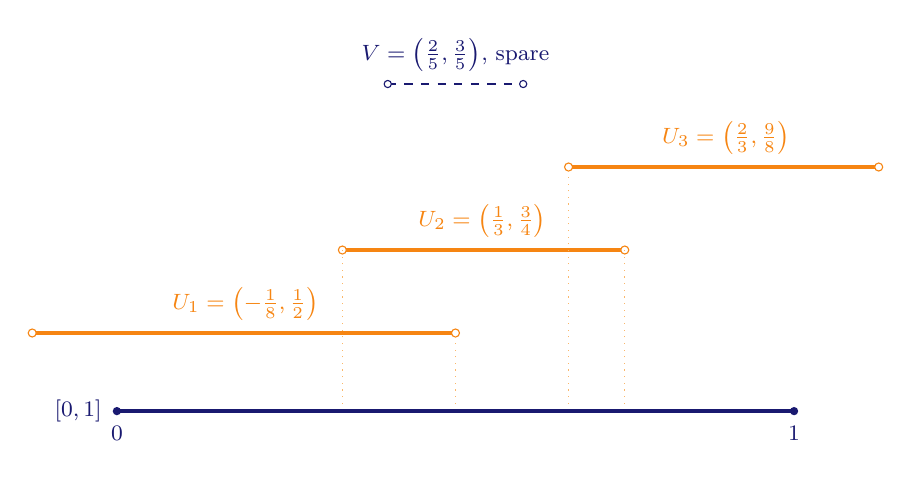
\begin{tikzpicture}[x=8.6cm,y=0.62cm,every node/.style={font=\footnotesize}]
  % The compact segment.
  \draw[MidnightBlue,line width=1.5pt] (0,0) -- (1,0);
  \fill[MidnightBlue] (0,0) circle (1.5pt);
  \fill[MidnightBlue] (1,0) circle (1.5pt);
  \node[below=2pt,MidnightBlue] at (0,0) {$0$};
  \node[below=2pt,MidnightBlue] at (1,0) {$1$};
  \node[left=2pt,MidnightBlue] at (0,0) {$[0,1]$};
  % Three open intervals that already cover [0,1].
  \draw[BurntOrange,line width=1.7pt] (-0.125,1.6) -- (0.50,1.6);
  \draw[BurntOrange,fill=white] (-0.125,1.6) circle (1.45pt);
  \draw[BurntOrange,fill=white] (0.50,1.6) circle (1.45pt);
  \node[above=1pt,BurntOrange] at (0.19,1.6) {$U_1=\bigl(-\frac18,\frac12\bigr)$};
  \draw[BurntOrange,line width=1.7pt] (0.333,3.3) -- (0.75,3.3);
  \draw[BurntOrange,fill=white] (0.333,3.3) circle (1.45pt);
  \draw[BurntOrange,fill=white] (0.75,3.3) circle (1.45pt);
  \node[above=1pt,BurntOrange] at (0.54,3.3) {$U_2=\bigl(\frac13,\frac34\bigr)$};
  \draw[BurntOrange,line width=1.7pt] (0.667,5.0) -- (1.125,5.0);
  \draw[BurntOrange,fill=white] (0.667,5.0) circle (1.45pt);
  \draw[BurntOrange,fill=white] (1.125,5.0) circle (1.45pt);
  \node[above=1pt,BurntOrange] at (0.90,5.0) {$U_3=\bigl(\frac23,\frac98\bigr)$};
  % One member of the cover that the finite subcover does not use.
  \draw[MidnightBlue,dashed,thin] (0.40,6.7) -- (0.60,6.7);
  \draw[MidnightBlue,fill=white] (0.40,6.7) circle (1.3pt);
  \draw[MidnightBlue,fill=white] (0.60,6.7) circle (1.3pt);
  \node[above=1pt,MidnightBlue] at (0.50,6.7) {$V=\bigl(\frac25,\frac35\bigr)$, spare};
  % Overlaps that let the three intervals meet.
  \draw[BurntOrange!55,dotted] (0.333,0.15) -- (0.333,3.3);
  \draw[BurntOrange!55,dotted] (0.50,0.15) -- (0.50,1.6);
  \draw[BurntOrange!55,dotted] (0.667,0.15) -- (0.667,5.0);
  \draw[BurntOrange!55,dotted] (0.75,0.15) -- (0.75,3.3);
\end{tikzpicture}
